\section{Ex.1 2 FLPs 12 EPNs}
\textbf{Ticktime influence on the Blacklist algorithm with one fail-over.}
\\~\\
The results of the experiment are shown in table ~\ref{table:Ex1MitchResults}. It shows that there is a linear line going up with the amount of TFs lost compared to ticktime. It also shows that the mean and standard deviation at ticktime 20 are round. This would be because of the ticktime being in sync with the heartbeat rate.

\begin{table}[h!]
\caption*{\textbf{Experiment one (2/12) using a cluster of Raspberry Pi's}}
\begin{tabular}{| l | l | l |}
\hline
Ticktime & Mean TF loss & Standard Deviation \\ \hline
5 & 2.16 & 0.49 \\ \hline
10 & 2.13 & 0.47 \\ \hline
15 & 3.08 & 0.2 \\ \hline
20 & 3.0 & 0 \\ \hline
25 & 3.52 & 0.51 \\ \hline
30 & 4.32 & 0.57 \\ \hline
35 & 4.13 & 0.79 \\ \hline
40 & 4.56 & 0.16 \\ \hline
\end{tabular}
\caption{Results of the TFs lost with 1 fail over using a cluster of Raspberry Pi's}
\label{table:Ex1MitchResults}
\end{table}

~\\ If we compare this to the previous experiment shown in table ~\ref{table:Ex1HeikoResults}, we can see that there is a small difference in the mean of the TFs lost, and some small variations in the standard deviation.

\begin{table}[h!]
\caption*{\textbf{Experiment one (2/12) using a cluster on Nikhef}}
\begin{tabular}{| l | l | l |}
\hline
Ticktime & Mean TF loss & Standard Deviation \\ \hline
5 & 1.24 & 0.4271 \\ \hline
10 & 1.84 & 0.731 \\ \hline
15 & 2.16 & 0.3666 \\ \hline
20 & 2.12 & 0.325 \\ \hline
25 & 2.708 & 0.4545 \\ \hline
30 & 3 & 0 \\ \hline
35 & 3.52 & 4.996 \\ \hline
40 & 3.76 & 0.4271 \\ \hline
\end{tabular}
\caption{Results of the TFs lost with 1 fail over using a cluster of Intel Xeons (van der Heijden, 2018, p. 36)}
\label{table:Ex1HeikoResults}
\end{table}

\section{Ex.2 2 FLPs 12 EPNs}
\textbf{Ticktime influence on the Blacklist algorithm with all but one fail-over.}
\\~\\
Table ~\ref{table:Ex2MitchResults} shows the lost TFs per ticktime/EPN ratio. For every extra EPN that is lost, the lost TFs increase in a linear motion. This is compliant with the previous experiment. These results are shown in table ~\ref{table:Ex2HeikoResults}. A histogram of ticktime 5 shown at ~\ref{Ex2Histogram} shows that the standard deviation is 0.9568.

\begin{table}[h!]
\caption*{\textbf{Experiment two (2/12) using a cluster of Raspberry Pi's}}
\resizebox{\textwidth}{!}{\begin{tabular}{| p{0.1\linewidth} | >{\centering}m{0.7cm} | >{\centering}m{0.7cm} | >{\centering}m{0.7cm} | >{\centering}m{0.7cm} | >{\centering}m{0.7cm} | >{\centering}m{0.7cm} | >{\centering}m{0.7cm} | >{\centering}m{0.7cm} | >{\centering}m{0.7cm} | >{\centering}m{0.7cm} | >{\centering}m{0.7cm} | >{\centering}m{0.7cm} |}
\hline
Lost EPNs & 1 EPN & 2 EPNs & 3 EPNs & 4 EPNs & 5 EPNs & 6 EPNs & 7 EPNs & 8 EPNs & 9 EPNs & 10 EPNs & 11 EPNs & Total \tabularnewline \hline
Ticktime &&&&&&&&&&&& \tabularnewline \hline
5 & 2 & 1.92 & 1.96 & 1.92 & 1.92 & 2.08 & 2.63 & 2.92 & 3.21 & 3.71 & 4.67 & \textbf{18.92}\tabularnewline \hline
10 & 2 & 2.36 & 2.6 & 3.2 & 3.08 & 3.04 & 3.08 & 3.72 & 4.04 & 5.08 & 6.68 & \textbf{28.88} \tabularnewline \hline
15 & 2.96 & 2.96 & 2.96 & 3 & 3.58 & 3.58 & 3.96 & 4.38 & 5.25 & 6.38 & 8.54 & \textbf{37.54}\tabularnewline \hline
20 & 2.96 & 3.13 & 3.25 & 3.75 & 4 & 4.29 & 4.67 & 5.46 & 6.29 & 8.04 & 10.38 & \textbf{46.67}\tabularnewline \hline
25 & 3.36 & 3.64 & 3.92 & 4 & 4.56 & 4.96 & 5.44 & 6.32 & 7.4 & 9 & 12.68 & \textbf{55.28}\tabularnewline \hline
\end{tabular}}
\caption{Cumulative lost TFs by ticktime/EPN ratio with a flat sample size for the Blacklist algorithm}
\label{table:Ex2MitchResults}
\end{table}

\begin{table}[h!]
\caption*{\textbf{Experiment two (2/12) using a cluster on Nikhef}}
\resizebox{\textwidth}{!}{\begin{tabular}{| p{0.1\linewidth} | >{\centering}m{0.7cm} | >{\centering}m{0.7cm} | >{\centering}m{0.7cm} | >{\centering}m{0.7cm} | >{\centering}m{0.7cm} | >{\centering}m{0.7cm} | >{\centering}m{0.7cm} | >{\centering}m{0.7cm} | >{\centering}m{0.7cm} | >{\centering}m{0.7cm} | >{\centering}m{0.7cm} |}
\hline
Lost EPNs & 1 EPN & 2 EPNs & 3 EPNs & 4 EPNs & 5 EPNs & 6 EPNs & 7 EPNs & 8 EPNs & 9 EPNs & 10 EPNs & 11 EPNs \tabularnewline \hline
Ticktime &&&&&&&&&&& \tabularnewline \hline
5 & 1 & 2 & 2 & 2 & 2 & 2 & 2 & 3 & 3 & 3 & 4 \tabularnewline \hline
10 & 1 & 2 & 3 & 3 & 3 & 3 & 3 & 3 & 4 & 4 & 5 \tabularnewline \hline
15 & 1 & 3 & 3 & 3 & 3 & 3 & 4 & 4 & 4 & 5 & 7 \tabularnewline \hline
20 & 9 & 3 & 3 & 3 & 4 & 4 & 4 & 5 & 5 & 6 & 8 \tabularnewline \hline
25 & 11 & 3 & 4 & 4 & 4 & 4 & 5 & 5 & 6 & 7 & 9 \tabularnewline \hline
\end{tabular}}
\caption{Cumulative lost TFs by ticktime by lost EPNs (van der Heijden, 2018, p. 38)}
\label{table:Ex2HeikoResults}
\end{table}

\newpage

\begin{figure}[h!]
	\centering
	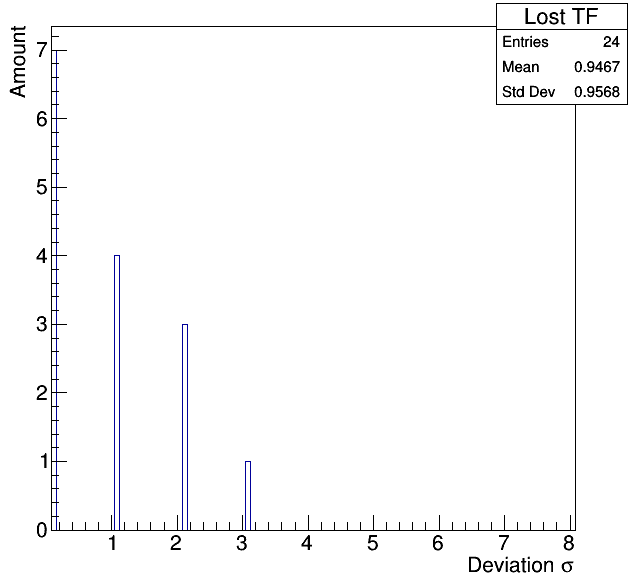
\includegraphics[scale=0.5]{./graphics/ex2_histogram.png}
	\caption{Histogram of the TF lost for ticktime 5}
	\label{Ex2Histogram}
\end{figure}

\newpage

\section{Ex.3 2 FLPs 12 EPNs}
\textbf{Ticktime influence on the Blacklist algorithm with all but one-fail over with random sample size.}
\\~\\
Compliant with the previous results, the TF loss to ticktime ratio rises in a linear line, with no absurdities along the way. The amounts are also negligibly different to the previous results. Results can be seen in table ~\ref{table:Ex3MitchResults} and table ~\ref{table:Ex3HeikoResults}. A histogram for ticktime 5 can be seen at ~\ref{fig:Ex3Histogram}. It shows a standard deviation of 1.569 for all the TFs lost in the entire run. 

\begin{table}[h!]
\caption*{\textbf{Experiment three (2/12) using a cluster of Raspberry Pi's}}
\resizebox{\textwidth}{!}{\begin{tabular}{| p{0.1\linewidth} | >{\centering}m{0.7cm} | >{\centering}m{0.7cm} | >{\centering}m{0.7cm} | >{\centering}m{0.7cm} | >{\centering}m{0.7cm} | >{\centering}m{0.7cm} | >{\centering}m{0.7cm} | >{\centering}m{0.7cm} | >{\centering}m{0.7cm} | >{\centering}m{0.7cm} | >{\centering}m{0.7cm} | >{\centering}m{0.7cm} |}
\hline
Lost EPNs & 1 EPN & 2 EPNs & 3 EPNs & 4 EPNs & 5 EPNs & 6 EPNs & 7 EPNs & 8 EPNs & 9 EPNs & 10 EPNs & 11 EPNs & Total \tabularnewline \hline
Ticktime &&&&&&&&&&&& \tabularnewline \hline
5 & 1.92 & 1.96 & 1.96 & 2.2 & 2.52 & 2.88 & 2.96 & 3.08 & 3.56 & 4.2 & 4.92 & \textbf{23.88}\tabularnewline \hline
10 & 1.96 & 2.3 & 2.52 & 2.74 & 2.81 & 2.93 & 2.85 & 3.48 & 3.85 & 4.74 & 6.33 & \textbf{26.52}\tabularnewline \hline
15 & 3 & 2.92 & 2.96 & 2.96 & 3.21 & 3.38 & 4.04 & 4.42 & 5.25 & 6.29 & 8.67 & \textbf{37.08}\tabularnewline \hline
20 & 3 & 3 & 3.38 & 3.5 & 3.92 & 4.17 & 4.79 & 5.17 & 6.08 & 7.54 & 10.88 & \textbf{45.12}\tabularnewline \hline
25 & 3.71 & 3.54 & 3.92 & 3.83 & 4.13 & 4.79 & 5.33 & 6.13 & 7.21 & 9.17 & 13.38 & \textbf{55.13}\tabularnewline \hline
\end{tabular}}
\caption{Cumulative lost TFs by ticktime/EPN ratio with a random sample size for the Blacklist algorithm}
\label{table:Ex3MitchResults}
\end{table}

\begin{table}[htb]
\caption*{\textbf{Experiment three (2/12) using a cluster on Nikhef}}
\resizebox{\textwidth}{!}{\begin{tabular}{| p{0.1\linewidth} | >{\centering}m{0.7cm} | >{\centering}m{0.7cm} | >{\centering}m{0.7cm} | >{\centering}m{0.7cm} | >{\centering}m{0.7cm} | >{\centering}m{0.7cm} | >{\centering}m{0.7cm} | >{\centering}m{0.7cm} | >{\centering}m{0.7cm} | >{\centering}m{0.7cm} | >{\centering}m{0.7cm} |}
\hline
Lost EPNs & 1 EPN & 2 EPNs & 3 EPNs & 4 EPNs & 5 EPNs & 6 EPNs & 7 EPNs & 8 EPNs & 9 EPNs & 10 EPNs & 11 EPNs \tabularnewline \hline
Ticktime &&&&&&&&&&& \tabularnewline \hline
5 & 1 & 2 & 2 & 2 & 2 & 3 & 3 & 3 & 3 & 4 & 4 \tabularnewline \hline
10 & 1 & 3 & 3 & 3 & 3 & 3 & 3 & 4 & 4 & 5 & 6 \tabularnewline \hline
15 & 11 & 3 & 3 & 3 & 3 & 3 & 4 & 4 & 5 & 6 & 7 \tabularnewline \hline
20 & 10 & 3 & 3 & 3 & 4 & 4 & 4 & 5 & 6 & 7 & 9 \tabularnewline \hline
25 & 13 & 3 & 4 & 4 & 4 & 4 & 5 & 5 & 7 & 8 & 10 \tabularnewline \hline
\end{tabular}}
\caption{Cumulative TF data loss across events with the Blacklist algorithm and a random sample size (van der Heijden, 2018, p. 40)} 
\label{table:Ex3HeikoResults}
\end{table}

\begin{figure}
	\centering
	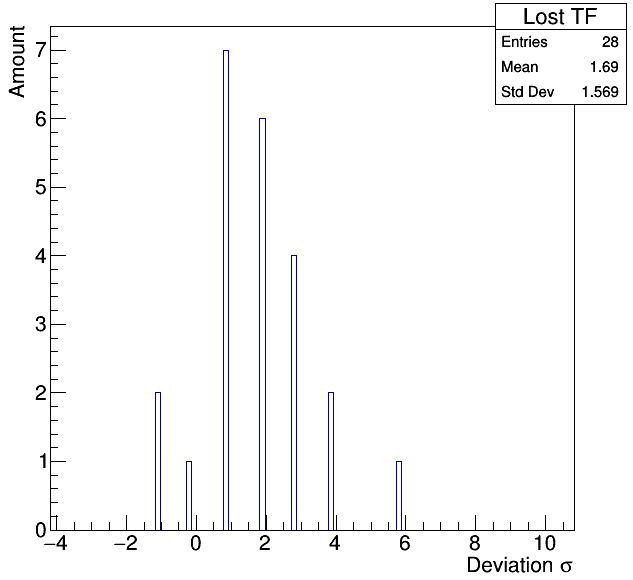
\includegraphics[scale=0.5]{./graphics/ex3_histogram.png}
	\caption{Histogram of the TF loss for ticktime 5}
	\label{fig:Ex3Histogram}
\end{figure}

\newpage

\section{Ex.1 3 FLPs 18 EPNs}
\textbf{Ticktime influence on the Blacklist algorithm with one fail-over.}
\\~\\
The results of the experiment are shown in table ~\ref{table:Ex1318Results}. It shows a linear line going up. At ticktime 10 there is only an average of 1 TF loss. This is the 1 TF that is lost when a shutdown is initialized. These results are lower compared to the results in table ~\ref{table:Ex1MitchResults}.

\begin{table}[h!]
\caption*{\textbf{Experiment one (3/18) using a cluster of Raspberry Pi's}}
\begin{tabular}{| l | l | l |}
\hline
Ticktime & Mean TF loss & Standard Deviation \\ \hline
5 & 1.13 & 0.34 \\ \hline
10 & 1 & 0 \\ \hline
15 & 1.92 & 0.50 \\ \hline
20 & 2.08 & 0.28 \\ \hline
25 & 2.08 & 0.28 \\ \hline
30 & 2.08 & 0.28 \\ \hline
35 & 2.52 & 0.51 \\ \hline
40 & 2.84 & 0.37 \\ \hline
\end{tabular}
\caption{Results of the TFs lost with 1 fail over using a cluster of Raspberry Pi's}
\label{table:Ex1318Results}
\end{table}

\newpage

\section{Ex.2 3 FLPs 18 EPNs}
\textbf{Ticktime influence on the Blacklist algorithm with all but one fail-over.}
\\~\\
The results of the experiment are shown in ~\ref{table:Ex2318Results}. It shows a lower TF loss compared to ~\ref{table:Ex2MitchResults}. It shows that at a ticktime of 5, every fail over will have a TF loss of < 2. This 1 TF comes from the shutdown signal. This means that the time between shutdown, and coming back around again to the EPN, is longer than the time needed to refresh the blacklist. 

\begin{table}[h!]
\caption*{\textbf{Experiment two (3/18) using a cluster of Raspberry Pi's}}
\resizebox{\textwidth}{!}{\begin{tabular}{| p{0.1\linewidth} | >{\centering}m{0.7cm} | >{\centering}m{0.7cm} | >{\centering}m{0.7cm} | >{\centering}m{0.7cm} | >{\centering}m{0.7cm} | >{\centering}m{0.7cm} | >{\centering}m{0.7cm} | >{\centering}m{0.7cm} | >{\centering}m{0.7cm} | >{\centering}m{0.7cm} | >{\centering}m{0.7cm} | >{\centering}m{0.7cm} |}
\hline
Lost EPNs & 1 EPN & 2 EPNs & 3 EPNs & 4 EPNs & 5 EPNs & 6 EPNs & 7 EPNs & 8 EPNs & 9 EPNs & 10 EPNs & 11 EPNs & Total \tabularnewline \hline
Ticktime &&&&&&&&&&&& \tabularnewline \hline
5 & 1.14 & 1.1 & 1.05 & 1.05 & 1.05 & 1.1 & 1.5 & 1 & 1.67 & 1.52 & 1.62 & \textbf{3.33}\tabularnewline \hline
10 & 1.04 & 1.25 & 1.29 & 1.17 & 1.88 & 2.04 & 2 & 2.08 & 1.96 & 2.08 & 2.04 & \textbf{8.83} \tabularnewline \hline
15 & 2 & 2.08 & 2.08 & 2.08 & 2.04 & 2 & 2.08 & 2.08 & 2.33 & 2.71 & 2.79 & \textbf{14.29}\tabularnewline \hline
20 & 2.16 & 2.12 & 2.08 & 2.08 & 2.16 & 2.12 & 2.4 & 2.52 & 2.96 & 3.04 & 3.08 & \textbf{16.72}\tabularnewline \hline
25 & 2.04 & 2.16 & 2.04 & 2.16 & 2.6 & 2.48 & 2.92 & 3.08 & 3.2 & 3.36 & 3.72 & \textbf{19.76}\tabularnewline \hline
\end{tabular}}
\caption{Cumulative lost TFs by ticktime/EPN ratio with a flat sample size for the Blacklist algorithm}
\label{table:Ex2318Results}
\end{table}

\section{Ex.3 3 FLPs 18 EPNs}
\textbf{Ticktime influence on the Blacklist algorithm with all but one-fail over with random sample size.}
\\~\\

The results of the experiment are shown in table ~\ref{table:Ex3318Results}. Oddly enough these results show a more sine wave in the data loss. All these results are again lower compared to ~\ref{table:Ex3MitchResults}.

\begin{table}[h!]
\caption*{\textbf{Experiment three (3/18) using a cluster of Raspberry Pi's}}
\resizebox{\textwidth}{!}{\begin{tabular}{| p{0.1\linewidth} | >{\centering}m{0.7cm} | >{\centering}m{0.7cm} | >{\centering}m{0.7cm} | >{\centering}m{0.7cm} | >{\centering}m{0.7cm} | >{\centering}m{0.7cm} | >{\centering}m{0.7cm} | >{\centering}m{0.7cm} | >{\centering}m{0.7cm} | >{\centering}m{0.7cm} | >{\centering}m{0.7cm} | >{\centering}m{0.7cm} |}
\hline
Lost EPNs & 1 EPN & 2 EPNs & 3 EPNs & 4 EPNs & 5 EPNs & 6 EPNs & 7 EPNs & 8 EPNs & 9 EPNs & 10 EPNs & 11 EPNs & Total \tabularnewline \hline
Ticktime &&&&&&&&&&&& \tabularnewline \hline
5 & 2.56 & 2.39 & 2.22 & 1.17 & 1.22 & 2 & 1.11 & 2.17 & 1.44 & 1.33 & 1.72 & \textbf{9.33}\tabularnewline \hline
10 & 2.88 & 2.88 & 2.38 & 1.08 & 1.71 & 2 & 1.54 & 2.25 & 2.08 & 2 & 2.29 & \textbf{13.08}\tabularnewline \hline
15 & 3.08 & 4 & 3 & 2.04 & 2.04 & 2.58 & 2.08 & 3.04 & 2.33 & 2.25 & 2.54 & \textbf{19}\tabularnewline \hline
20 & 3.28 & 4.04 & 3.24 & 2.08 & 2.12 & 3.12 & 2.16 & 3.16 & 3 & 2.88 & 3.08 & \textbf{22.16}\tabularnewline \hline
25 & 3.7 & 4.09 & 3.87 & 2.52 & 2.78 & 3.13 & 2.83 & 3.65 & 3.39 & 3.3 & 3.96 & \textbf{27.22}\tabularnewline \hline
\end{tabular}}
\caption{Cumulative lost TFs by ticktime/EPN ratio with a random sample size for the Blacklist algorithm}
\label{table:Ex3318Results}
\end{table}

\newpage

\section{Ex.1 4 FLPs 24 EPNs}
\textbf{Ticktime influence on the Blacklist algorithm with one fail-over.}
\\~\\

\begin{table}[h!]
\caption*{\textbf{Experiment one (4/24) using a cluster of Raspberry Pi's}}
\begin{tabular}{| l | l | l |}
\hline
Ticktime & Mean TF loss & Standard Deviation \\ \hline
5 & 1 & 0 \\ \hline
10 & 1.08 & 0.28 \\ \hline
15 & 1.76 & 0.53 \\ \hline
20 & 2.12 & 0.44 \\ \hline
25 & 2 & 0 \\ \hline
30 & 2 & 0 \\ \hline
35 & 2.16 & 0.37 \\ \hline
40 & 2.33 & 0.48 \\ \hline
\end{tabular}
\caption{Results of the TFs lost with 1 fail over using a cluster of Raspberry Pi's}
\label{table:Ex1424Results}
\end{table}

\section{Ex.2 4 FLPs 24 EPNs}
\textbf{Ticktime influence on the Blacklist algorithm with all but one fail-over.}
\\~\\
Table ~\ref{table:Ex1424Results} shows the results of the experiment. It shows a the same linear line going up per EPN as in the previous experiments. These results are yet again smaller than the results from table ~\ref{table:Ex1318Results}.

\begin{table}[h!]
\caption*{\textbf{Experiment two (4/24) using a cluster of Raspberry Pi's}}
\resizebox{\textwidth}{!}{\begin{tabular}{| p{0.1\linewidth} | >{\centering}m{0.7cm} | >{\centering}m{0.7cm} | >{\centering}m{0.7cm} | >{\centering}m{0.7cm} | >{\centering}m{0.7cm} | >{\centering}m{0.7cm} | >{\centering}m{0.7cm} | >{\centering}m{0.7cm} | >{\centering}m{0.7cm} | >{\centering}m{0.7cm} | >{\centering}m{0.7cm} | >{\centering}m{0.7cm} |}
\hline
Lost EPNs & 1 EPN & 2 EPNs & 3 EPNs & 4 EPNs & 5 EPNs & 6 EPNs & 7 EPNs & 8 EPNs & 9 EPNs & 10 EPNs & 11 EPNs & Total \tabularnewline \hline
Ticktime &&&&&&&&&&&& \tabularnewline \hline
5 & 1.15 & 1.15 & 1.25 & 1.15 & 1.05 & 1.15 & 1.15 & 1.15 & 1.1 & 1.1 & 1.25 & \textbf{2.65}\tabularnewline \hline
10 & 1.08 & 1.04 & 1.08 & 1.08 & 1.48 & 1.48 & 1.52 & 1.8 & 2.04 & 1.96 & 2.24 & \textbf{6.8} \tabularnewline \hline
15 & 1.4 & 1.68 & 1.72 & 2 & 2.04 & 2.04 & 2.08 & 2 & 2.08 & 2 & 2.08 & \textbf{11.12}\tabularnewline \hline
20 & 2.12 & 2.04 & 2.08 & 2 & 2.16 & 2.12 & 2.08 & 2.08 & 2.12 & 2.08 & 2.24 & \textbf{13.12}\tabularnewline \hline
25 & 2.12 & 2.12 & 2.16 & 2.12 & 2.12 & 2.04 & 2.2 & 2.08 & 2.6 & 2.68 & 2.64 & \textbf{14.88}\tabularnewline \hline
\end{tabular}}
\caption{Cumulative lost TFs by ticktime/EPN ratio with a flat sample size for the Blacklist algorithm}
\label{table:Ex2424Results}
\end{table}

\section{Ex.3 4 FLPs 24 EPNs}
\textbf{Ticktime influence on the Blacklist algorithm with all but one fail-over with random sample size.}
\\~\\

\begin{table}[h!]
\caption*{\textbf{Experiment three (4/24) using a cluster of Raspberry Pi's}}
\resizebox{\textwidth}{!}{\begin{tabular}{| p{0.1\linewidth} | >{\centering}m{0.7cm} | >{\centering}m{0.7cm} | >{\centering}m{0.7cm} | >{\centering}m{0.7cm} | >{\centering}m{0.7cm} | >{\centering}m{0.7cm} | >{\centering}m{0.7cm} | >{\centering}m{0.7cm} | >{\centering}m{0.7cm} | >{\centering}m{0.7cm} | >{\centering}m{0.7cm} | >{\centering}m{0.7cm} |}
\hline
Lost EPNs & 1 EPN & 2 EPNs & 3 EPNs & 4 EPNs & 5 EPNs & 6 EPNs & 7 EPNs & 8 EPNs & 9 EPNs & 10 EPNs & 11 EPNs & Total \tabularnewline \hline
Ticktime &&&&&&&&&&&& \tabularnewline \hline
5 & 1.1 & 2.14 & 1.14 & 1.57 & 1.24 & 2.14 & 1.14 & 2 & 2.1 & 1.48 & 2.05 & \textbf{8.1}\tabularnewline \hline
10 & 1.52 & 1.96 & 1.04 & 1.68 & 1.4 & 2.04 & 1.36 & 1.88 & 2.04 & 2.04 & 2.16 & \textbf{9.12}\tabularnewline \hline
15 & 2.08 & 2.04 & 1.04 & 2.16 & 2.16 & 2.4 & 2.12 & 1.92 & 2.12 & 2.08 & 2.28 & \textbf{12.4}\tabularnewline \hline
20 & 2.04 & 2.2 & 1.48 & 2.32 & 2.16 & 2.88 & 2.04 & 2.8 & 2.96 & 2.2 & 2.96 & \textbf{16.04}\tabularnewline \hline
25 & 2.13 & 2.54 & 2.08 & 2.33 & 2.33 & 3.13 & 2.13 & 2.96 & 3 & 2.92 & 3.04 & \textbf{18.58}\tabularnewline \hline
\end{tabular}}
\caption{Cumulative lost TFs by ticktime/EPN ratio with a random sample size for the Blacklist algorithm}
\label{table:Ex3424Results}
\end{table}

\section{Ex.4 4 FLPs 24 EPNs}
\textbf{Ticktime influence on the Blacklist algorithm with a fixed cluster fail-over pattern using a random sample size.}
\\~\\
Table ~\ref{table:Ex4424Results} shows the results of the experiment. It shows that for the first 4 clusters the TF loss is low, but for the last cluster it's substantially higher. Because of this, the total average is also a lot higher.

\begin{table}[h!]
\caption*{\textbf{Experiment four (4/24) using a cluster of Raspberry Pi's}}
\resizebox{\textwidth}{!}{\begin{tabular}{| >{\centering}m{2cm} | >{\centering}m{2cm} | >{\centering}m{2cm} | >{\centering}m{2cm} | >{\centering}m{2cm} | >{\centering}m{2cm} | >{\centering}m{2cm} |}
\hline
Lost Clusters & 1 Cluster & 2 Clusters & 3 Clusters & 4 Clusters & 5 Clusters & Total \tabularnewline \hline
Ticktime &&&&&& \tabularnewline \hline
5 & 2.83 & 5.25 & 1.88 & 4.67 & 250.67 & \textbf{261.29}\tabularnewline \hline
10 & 3.64 & 3.76 & 6.04 & 4.52 & 285.92 & \textbf{299.88}\tabularnewline \hline
15 & 5.6 & 2.04 & 6.28 & 7.76 & 277.68 & \textbf{295.36}\tabularnewline \hline
20 & 7.26 & 4.74 & 6.26 & 13.3 & 296.09 & \textbf{323.65}\tabularnewline \hline
25 & 7.44 & 8.4 & 8.12 & 9.44 & 254.72 & \textbf{284.12}\tabularnewline \hline
\end{tabular}}
\caption{Cumulative lost TFs by ticktime/EPN ratio with a random sample size for the Blacklist algorithm and a fixed cluster 	fail-over pattern}
\label{table:Ex4424Results}
\end{table}

\section{Ex.5 4 FLPs 24EPNs}
\textbf{Ticktime influence on the Blacklist algorithm with a random cluster fail-over pattern using a random sample size}
\\~\\
Table ~\ref{table:Ex5424Results} shows the result of the experiment. It shows that with a random cluster fail-over pattern, the total average TF loss is close to the results in table ~\ref{table:Ex4424Results}, but for each seperate cluster they are higher. Unlike the previous experiment where it's all lower numbers first and then finally a very large one.

\begin{table}[h!]
\caption*{\textbf{Experiment five (4/24) using a cluster of Raspberry Pi's}}
\resizebox{\textwidth}{!}{\begin{tabular}{| >{\centering}m{2cm} | >{\centering}m{2cm} | >{\centering}m{2cm} | >{\centering}m{2cm} | >{\centering}m{2cm} | >{\centering}m{2cm} | >{\centering}m{2cm} |}
\hline
Lost Clusters & 1 Cluster & 2 Clusters & 3 Clusters & 4 Clusters & 5 Clusters & Total \tabularnewline \hline
Ticktime &&&&&& \tabularnewline \hline
5 & 3.21 & 23.53 & 38.32 & 79.53 & 174.89 & \textbf{315.47}\tabularnewline \hline
10 & 4.48 & 21.92 & 35.36 & 40.44 & 185.04 & \textbf{283.24}\tabularnewline \hline
15 & 5.52 & 23 & 36.84 & 28.16 & 188.4 & \textbf{277.92}\tabularnewline \hline
20 & 5.68 & 24.8 & 39.6 & 42.52 & 190.64 & \textbf{299.24}\tabularnewline \hline
25 & 6.26 & 26.74 & 42.83 & 84.61 & 194.39 & \textbf{350.83}\tabularnewline \hline
\end{tabular}}
\caption{Cumulative lost TFs by ticktime/EPN ratio with a random sample size for the Blacklist algorithm and a fixed cluster 	fail-over pattern}
\label{table:Ex5424Results}
\end{table}

\section{Analysis}
\subsection{Comparison to the previous experiment}
To calculate the validity of the results, the Pearson correlation will be used. This is calculated using:\\
\begin{flalign*}
\hspace*{-5cm} \rho x,y = \frac{\sum (x-m_{x})(y-m_{y})}{\sqrt{\sum(x-m_{x})^2(y-m_{y})^2}}
\end{flalign*}

~\\ Where $m_{x}$ is the mean of vector $x$, and $m_{y}$ is the mean of vector $y$.
~\\ A way to calculate this in python is shown in listing ~\ref{lst:PearsonInPython} The results of this can be found in table ~\ref{table:PearsonCor}. The totals of all separate tests are combined to calculate this correlation. If the Pearson correlation is close to 1, it means that there is a strong positve linear correlation. If it's 0 then there is no linear correlation. If it's -1 then there is a strong negative linear correlation.

\begin{lstlisting}[frame=single,language=Python,caption={Pearson correlation calculation in Python},label={lst:PearsonInPython}]
from scipy.stats.stats import pearsonr
def list of values X
def list of values Y
pearsonr(X,Y)
\end{lstlisting}

\begin{table}[h!]
\begin{tabular}{| l | l | l |}
\hline
Experiment & Pearson Correlation \\ \hline
1 & 0.95 \\ \hline
2 & 0.99 \\ \hline
3 & 0.99 \\ \hline
\end{tabular}
\caption{Pearson correlation between the raspberry pi cluster and the cluster on Nikhef}
\label{table:PearsonCor}
\end{table}

~\\ These correlations all strongly deny the null hypothesis, and thus there is some sort of statistical relationship. They also are close to 1, which means they are close to having a total positive linear correlation. Thus concluded that there is indeed a correlation between the setup on Nikhef, and the setup using Raspberry Pi's.

\subsection{Increasing the numbers of FLPs and EPNs}

\subsubsection*{Differences between 2/12 and 3/18}
Table ~\ref{table:Diff23ex1} shows that over all the ticktimes that are measured, there is an average difference of 1.41. Table ~\ref{table:Diff23ex2} shows that this difference is 24.87, and table ~\ref{table:Diff23ex3} shows that it is 19.39. This means that for every experiment conducted there are fewer TFs lost when the amount of units are increased.

\begin{table}[!htbp]
\begin{tabular}{| l | l | l | l | l |}
\hline
Experiment 1 & 2/12 & 3/18 & Nominal difference & \% difference \\ \hline
Ticktime &&&& \\ \hline
5 & 2.16 & 1.13 & 1.03 & -47.68 \\ \hline
10 & 2.13 & 1 & 1.13 & -53.05 \\ \hline
15 & 3.08 & 1.92 & 1.16 & -37.66 \\ \hline
20 & 3 & 2.08 & 0.92 & -30.67 \\ \hline
25 & 3.52 & 2.08 & 1.44 & -40.91 \\ \hline
30 & 4.32 & 2.08 & 2.24 & -51.85 \\ \hline
35 & 4.13 & 2.52 & 1.61 & -38.98 \\ \hline
40 & 4.56 & 2.84 & 1.72 & -37.72 \\ \hline \hline
Average &&& \textbf{1.41} & \textbf{-41.82} \\ \hline
\end{tabular}
\caption{Differences for experiment one using 2/12 and 3/18 ratio's}
\label{table:Diff23ex1}
\end{table}

\begin{table}[!htbp]
\begin{tabular}{| l | l | l | l | l |}
\hline
Experiment 2 & 2/12 & 3/18 & Nominal difference & \% difference \\ \hline
Ticktime &&&& \\ \hline
5 & 18.92 & 3.33 & 15.59 & -82.4 \\ \hline
10 & 28.88 & 8.83 & 20.05 & -68.43 \\ \hline
15 & 37.54 & 14.29 & 23.25 & -61.93 \\ \hline
20 & 46.67 & 16.72 & 29.95 & -64.17 \\ \hline
25 & 55.28 & 19.76 & 35.52 & -64.25 \\ \hline \hline
Average &&& \textbf{24.87} & \textbf{-66.4} \\ \hline
\end{tabular}
\caption{Differences for experiment two using 2/12 and 3/18 ratio's}
\label{table:Diff23ex2}
\end{table}

\begin{table}[!htbp]
\begin{tabular}{| l | l | l | l | l |}
\hline
Experiment 3 & 2/12 & 3/18 & Nominal difference & \% difference \\ \hline
Ticktime &&&& \\ \hline
5 & 23.88 & 9.33 & 14.55 & -60.93 \\ \hline
10 & 26.52 & 13.08 & 13.44 & -50.68 \\ \hline
15 & 37.08 & 19 & 18.08 & -48.76 \\ \hline
20 & 45.12 & 22.16 & 22.96 & -50.89 \\ \hline
25 & 55.13 & 27.22 & 27.91 & -50.63 \\ \hline \hline
Average &&& \textbf{19.39} & \textbf{-51.64} \\ \hline
\end{tabular}
\caption{Differences for experiment three using 2/12 and 3/18 ratio's}
\label{table:Diff23ex3}
\end{table}

\subsubsection*{Differences between 3/18 and 4/24}
Table ~\ref{table:Diff34ex1} shows that over all the ticktimes that are measured, there is an average difference of 0.15. Table ~\ref{table:Diff34ex2} shows that this difference is 2.87, and table ~\ref{table:Diff34ex3} shows that it is 5.31. These results yet again shows fewer TFs lost when the units are increased, though not as many as with the previous increase. Further increasing the units should inevitably level the amount of TFs lost to 1.

\begin{table}[!htbp]
\begin{tabular}{| l | l | l | l | l |}
\hline
Experiment 1 & 3/18 & 4/24 & Nominal difference & \% difference \\ \hline
Ticktime &&&& \\ \hline
5 & 1.13 & 1 & 0.13 & -11.5 \\ \hline
10 & 1 & 1.08 & -0.08 & 8 \\ \hline
15 & 1.92 & 1.76 & 0.16 & -8.33 \\ \hline
20 & 2.08 & 2.12 & -0.04 & 1.92 \\ \hline
25 & 2.08 & 2 & 0.08 & -3.85 \\ \hline
30 & 2.08 & 2 & 0.08 & -3.85 \\ \hline
35 & 2.52 & 2.16 & 0.36 & -14.29 \\ \hline
40 & 2.84 & 2.33 & 0.51 & -17.96 \\ \hline \hline
Average &&& \textbf{0.15} & \textbf{-7.67} \\ \hline
\end{tabular}
\caption{Differences for experiment one using 3/18 and 4/24 ratio's}
\label{table:Diff34ex1}
\end{table}

\begin{table}[!htbp]
\begin{tabular}{| l | l | l | l | l |}
\hline
Experiment 2 & 3/18 & 4/24 & Nominal difference & \% difference \\ \hline
Ticktime &&&& \\ \hline
5 & 3.33 & 2.65 & 0.68 & -20.42 \\ \hline
10 & 8.83 & 6.8 & 2.03 & -22.99 \\ \hline
15 & 14.29 & 11.12 & 3.17 & -22.18 \\ \hline
20 & 16.72 & 13.12 & 3.6 & -21.53 \\ \hline
25 & 19.76 & 14.88 & 4.88 & -24.7 \\ \hline \hline
Average &&& \textbf{2.87} & \textbf{-22.82} \\ \hline
\end{tabular}
\caption{Differences for experiment two using 3/18 and 4/24 ratio's}
\label{table:Diff34ex2}
\end{table}

\begin{table}[!htbp]
\begin{tabular}{| l | l | l | l | l |}
\hline
Experiment 3 & 3/18 & 4/24 & Nominal difference & \% difference \\ \hline
Ticktime &&&& \\ \hline
5 & 9.33 & 8.1 & 1.23 & -13.18 \\ \hline
10 & 13.08 & 9.12 & 3.96 & -30.28 \\ \hline
15 & 19.0 & 12.4 & 6.6 & -34.74 \\ \hline
20 & 22.16 & 16.04 & 6.12 & -27.62 \\ \hline
25 & 27.22 & 18.58 & 8.64 & -31.74 \\ \hline \hline
Average &&& \textbf{5.31} & \textbf{-29.24} \\ \hline
\end{tabular}
\caption{Differences for experiment three using 3/18 and 4/24 ratio's}
\label{table:Diff34ex3}
\end{table}

\newpage

\subsection{Comparing cluster fail-over patterns}
When comparing the data between the experiments, the t-test method is used. A way to implement a t-test analysis in Python is shown in listing ~\ref{lst:t-testinInPython}. For every increase in units the t-test will be performed.

\begin{lstlisting}[frame=single,language=Python,caption={t-test analysis in Python},label={lst:t-testinInPython}]
from scipy.stats import ttest_ind
def list of values X
def list of values Y
print ttest_ind(X, Y, equal_var=False)
\end{lstlisting}

~\\ The results are shown in ~\ref{table:Ttest45}. It shows that the t-statistic is -0.75 and the p-value is 0.474. This means that there is no significant statistical difference. Looking at the results it shows that that experiment four has lower values for the first four cluster fail-overs, but then has a higher value for the last cluster fail-over, whereas experiment five has higher values overall for each cluster fail-over. This shows that there is a difference in the lost TFs per individual cluster that has a fail-over depending on the layout, but that in the end the total amount is still similar.

\begin{table}[!htbp]
\begin{tabular}{| l | l | l | l | l |}
\hline
Ticktime & Experiment 4 & Experiment 5 & t-statistic & p-value \\ \hline
5 & 261.29 & 315.47 &  &  \\ \hline
10 & 299.88 & 283.24 &  &  \\ \hline
15 & 295.36 & 277.92 &  &  \\ \hline
20 & 323.65 & 299.24 &  &  \\ \hline
25 & 284.23 & 350.83 &  &  \\ \hline \hline
Total &  &  & \textbf{-0.75} & \textbf{0.474}\\ \hline
\end{tabular}
\caption{t-test results of experiment four and five}
\label{table:Ttest45}
\end{table}